%\VignetteIndexEntry{Interactive Interpretation of Linear Regression Models}
%\VignetteKeyword{termplot}
%\VignetteKeyword{interactive}
%\VignettePackage{LinRegInteractive}

\documentclass[nojss]{jss}

\usepackage{enumitem}
\usepackage{booktabs}
\usepackage{float}

%% need no \usepackage{Sweave}

\newcommand{\class}[1]{``\code{#1}''}
\newcommand{\quotes}[1]{``#1''}



%% almost as usual
\author{Martin Meermeyer\\ Universit\"at Wuppertal}
\Plainauthor{Martin Meermeyer}
\title{\pkg{LinRegInteractive}: An \proglang{R} Package for the Interactive Interpretation of Linear Regression Models}
\Plaintitle{LinRegInteractive: An R Package for the Interactive Interpretation of Linear Regression Models}
\Shorttitle{\pkg{LinRegInteractive}: Interactive Interpretation of Linear Regression Models} 

\Abstract{
To facilitate the interpretation of binary response and multiple linear regression models the package provides two major functions, \code{glm.interactive()} and \code{lm.interactive()}, which allow to observe the effects of variations of metric covariates in an interactive manner by means of termplots. 
Due to the interactive approach the functions provide an intuitive understanding of the mechanics of a particular model and are therefore especially useful for educational purposes.  
Technically the functions are based on the package \pkg{rpanel} and the only mandatory argument is an appropriate fitted-model object. Given this, the linear predictors, the marginal effects and, for models with binary outcomes, the probabilities are calculated automatically. For the marginal effects a numerical approach is used to handle nonlinear effects automatically. If there are two or more categorical covariates the corresponding effects are presented in a novel way. For publication purposes the user can customize the appearance of the termplots to a large extent. Tables capturing the model output and the effects can be printed to the \proglang{R} Console, optionally as copy-and-paste-ready \LaTeX-code. 
}
\Keywords{termplots, marginal effects, binary dependent variables}

%% publication information
%% NOTE: Typically, this can be left commented and will be filled out by the technical editor
%% \Volume{50}
%% \Issue{9}
%% \Month{June}
%% \Year{2012}
%% \Submitdate{2012-06-04}
%% \Acceptdate{2012-06-04}

%% The address of (at least) one author should be given
%% in the following format:
\Address{
  Martin Meermeyer\\
  Bergische Universit\"at Wuppertal\\
  Schumpeter School of Business and
  Economics\\
  Gaussstr.~20\\
  42119~Wuppertal, Germany\\
  E-mail: \email{meermeyer@statistik.uni-wuppertal.de}\\
  URL: \url{http://www.statistik.uni-wuppertal.de}\\
}

\begin{document}
\section{Introduction} \label{sec-intro}
The interpretation of the results for linear regression models with non-constant marginal effects can be tedious. For the multiple linear regression model this is the case when the covariates are incorporated in a nonparametric way. For binary response models this is true even for very simple linear link functions. As pointed out by \citet{Hoet2007} the interpretation of  binary response models becomes yet more complex, if
\begin{itemize} [leftmargin=1cm, rightmargin=0.5cm, label=$\bullet$]
\item more than one categorical covariate is contained in the model,
\item metric covariates are included nonparametrically,
\item interaction effects between metric and categorical covariates are included.
\end{itemize}
For the three mentioned cases the interpretation of the multiple linear regression model can be complex, too. Graphical displays of the effects are most often the best way to study the results of such models, especially in the presence of non-constant marginal effects.

The functions \code{glm.interactive()} and \code{lm.interactive()} facilitate the interpretation of binary response and multiple linear regression models by providing an interactive graphical presentation of the results. For each metric covariate the linear predictors, the marginal effects and, for models with binary responses, the probabilities can be displayed as termplots. The values of the other metric covariates can be adjusted interactively and for the specified covariate constellation tables of the effects can be printed to the console. Especially in case of the three circumstances mentioned above the functions are helpful in the following way:
\begin{itemize} [leftmargin=1cm, rightmargin=0.5cm, label=$\bullet$]
\item If more than one categorical variable is contained in the model, the effects in the termplots are calculated for every combination of factor levels. Each combination is referred to as \emph{group} and can be selected to be displayed or not.
\item For metric covariates which are incorporated nonparametrically the direct (analytical) calculation of the marginal effects is tedious. Therefore, these are calculated numerically with \code{splinefun()}.
\item The mechanics of interaction effects between metric and categorical covariates becomes obvious due to the separate treatment of the groups  and the interactive nature of the functions.
\end{itemize}

The function \code{glm.interactive()} was developed to translate suggestions for the interpretation of logit and probit models made by \citet{Hoet2007} into action, the \code{lm.interactive()} is a byproduct of this effort. The main purpose of these functions is to convey statistical concepts in educational contexts, \citet{Xie2013} gives a comprehensive overview of other recent approaches in this area. The implementation of the interactive GUI is based on the package \pkg{rpanel} \citep{BowmCrawAlex2007}. This package also contains an interactive teaching tool for spatial sampling which is described in detail in \citet{BowmGibsScot2010}. Printing \LaTeX-output to the console was inspired by the package \pkg{xtable} \citep{Dahl2012}, nevertheless an own implementation based on \code{format()} is used for technical reasons. The noninteractive visualization of the results for various types of regression models can be achieved with the package \pkg{effects} \citep{Fox2003}.

The remainder of the paper is structured as follows. In section~\ref{sec-quickstart} the basic usage of the main functions \code{glm.interactive()} and \code{lm.interactive()} is described. The benefits of the implemented  visualization approach are demonstrated by means of examples  in section~\ref{sec-visualization}.  Details of the text output produced by the \textit{Snapshot}-button are addressed in section~\ref{sec-output}. While the main focus of the functions relie on the interactive usage it is nevertheless easy to reproduce the results obtained by interaction. This is explained in section~\ref{sec-usage} and especially useful for publication purposes. For the same reason the format of the text output and the layout of the plots  can be controlled to a large extent by a number of non-mandatory arguments which is  described in-depth in section~\ref{subsec-custom-text} and \ref{subsec-custom-graph}. To achieve even more flexibility the fundamental layout of the plots can be specified in advance which is shown in section~\ref{subsec-predefine}. Additional arguments control the appearance of the GUI-panel which is addressed in section~\ref{subsec-custom-gui}. Fitted-model objects which do not inherit from \code{glm()} or \code{lm()} may be used as well. The requirements for the fitted-model objects are explained in section~\ref{sec-call-classes}. In this section also a workaround for problems with the raw data extraction is described.



\section{Quick start} \label{sec-quickstart}
In terms of mandatory arguments the interfaces of the functions are kept as simple as possible. For the function \code{glm.interactive()} only a fitted-model object of class \class{glm} and for \code{lm.interactive()} a fitted-model object of class \class{lm} must be passed.
For the fitted-model objects the following prerequisites must be met:
\begin{itemize} [leftmargin=1cm, rightmargin=0.5cm, label=$\bullet$]
\item  The model must contain at least one metric covariate.
\item The model must be specified with the formula interface and the data frame containing the variables must be passed with the \code{data} argument.
\item The categorical variables must be \code{factors} (ordered or unordered).
\item For \code{glm.interactive()}: the \code{family} of the fitted-model object must be \code{binomial}.
\end{itemize}

The functions may work as well for other classes of fitted-model objects. The requirements for this together with two examples are given in section~\ref{sec-call-classes}. Some formulas in the call of \code{glm()} or \code{lm()}  may cause a problem with the internal raw data extraction. A possible approach to solve this issue is also described in section~\ref{sec-call-classes}.

For a suitable fitted-model object the basic usage is simple. This is demonstrated by means of a probit model for defaults of consumer credits. The used dataset \code{creditdata}  is part of the package and was originally obtained from the \citet{DataCred2014}. A probit model with 3 metric covariates and 2 factors with 2 and 3 levels respectively is used as example:
%
\begin{Schunk}
\begin{Sinput}
 data("creditdata")
 model.2.fac <- glm(credit ~ amount + I(amount^2)  + age + duration*teleph  
     + housing, family = binomial(link="probit"), data = creditdata)
\end{Sinput}
\end{Schunk}
%

The variables are described in the documentation of the dataset \code{creditdata}.
Given the fitted-model object the start is simple:
%
\begin{Schunk}
\begin{Sinput}
 glm.interactive(model.2.fac) 
\end{Sinput}
\end{Schunk}
%

Users of the IDE \textbf{RStudio} may need to change the graphic device with \code{options(device = "x11")}  before calling the function because in current versions of \textbf{RStudio} multiple graphic devices occasionally do not work properly. After calling the function the basic handling is as follows:
\begin{enumerate}[leftmargin=1cm, rightmargin=0.5cm, label={\arabic{enumi}.}]
\item Select metric covariate to be displayed as termplot by using the dialog (see figure \ref{fig-001}, left). Within the IDE \textbf{RStudio} the selection dialog appears as text list in the integrated console (see figure \ref{fig-001}, right). 

\begin{figure}[ht]
\centering 
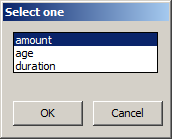
\includegraphics[height=3cm, width=3.712cm]{fig-001-1}  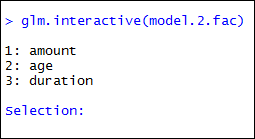
\includegraphics[height=3cm, width=5.504cm]{fig-001-2}
\caption{Initial dialog to select the metric covariate to be displayed.}
\label{fig-001}
\end{figure}

\item The GUI-panel (see figure~\ref{fig-002}, left) allows the following actions:
\begin{itemize} [leftmargin=0.5cm, rightmargin=0.5cm, label=$\bullet$]
\item The values of the metric covariates can be choosen by sliders. 
\item The type of the termplot to be displayed can be selected in the radiobox \textit{Type}.
\item If factors are present, the level-combinations of the factors to be displayed can be selected in the checkbox \textit{Groups}.
\item Tables of the effects can be printed to the \proglang{R Console} and optionally the actual plot is saved by pushing the button \textit{Snapshot}. The effects are calculated for the covariate constellation chosen by the sliders. 
\end{itemize}

\begin{figure}[ht]
\centering
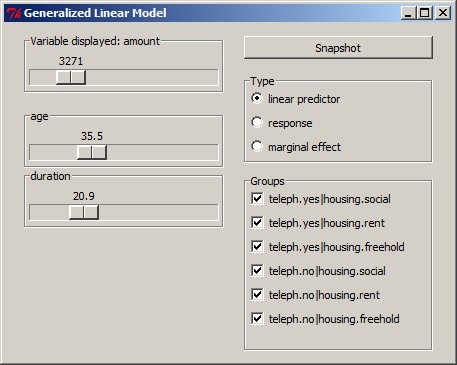
\includegraphics[height=5cm, width=6.26cm]{fig-002-1}   \quad 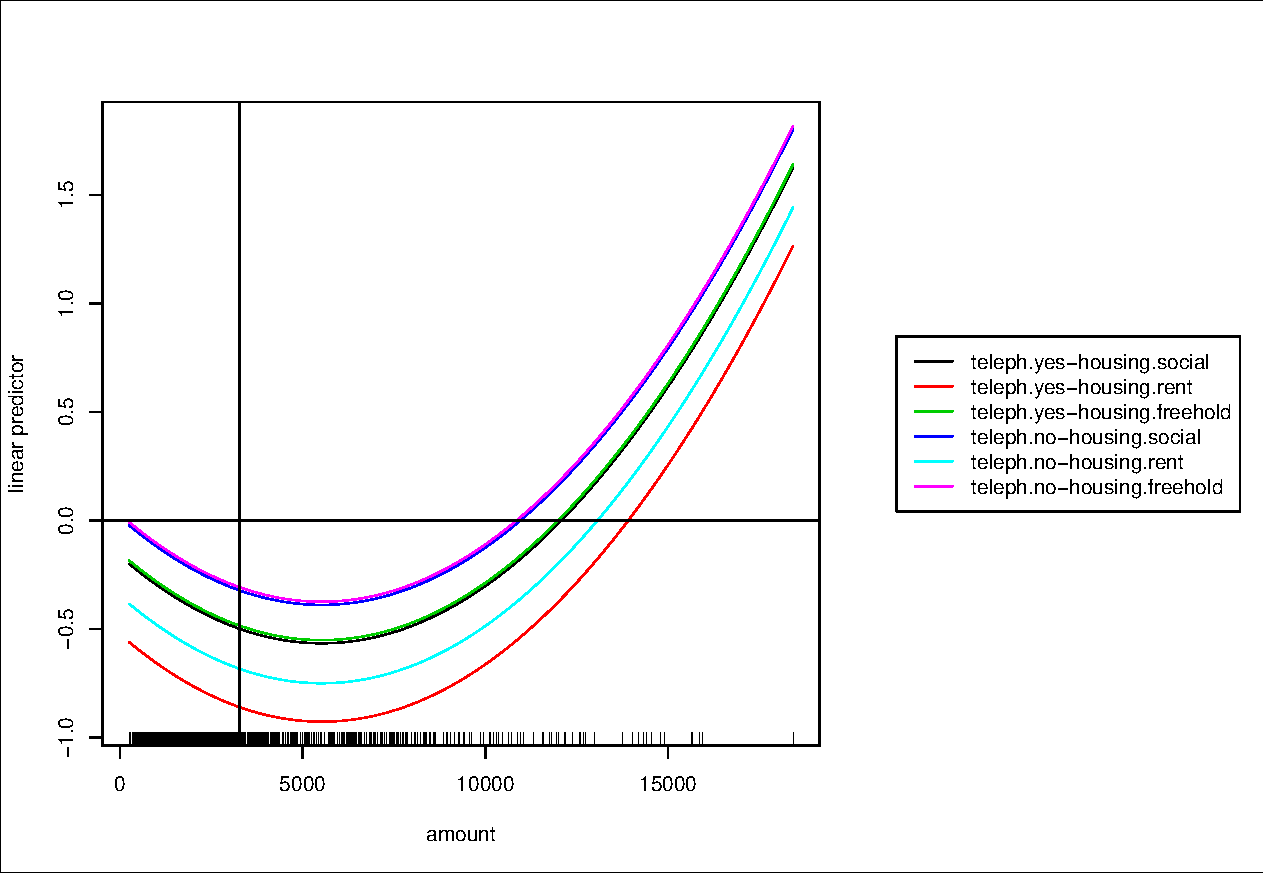
\includegraphics[height=5cm, width=7.233cm]{fig-002-2.pdf}
\caption{GUI-panel and initial termplot (linear predictor) of the selected metric covariate. By default the metric covariates are at their means and all groups are displayed.} \label{fig-002}
\end{figure}
\end{enumerate}

Details on the tables produced by the \textit{Snapshot}-button are explained in section~\ref{sec-output}.
On the right hand side of figure~\ref{fig-002} the initial termplot for the example model is shown.  The plot is optimized for screens and is reduced in size here to fit on the page, therefore the annotations may be hard to read. The termplots are calculated for the range of the selected metric covariate. The top slider controls the value of the selected metric covariate which is used to calculate the output triggered by the \emph{Snapshot}-button. The initial values of the sliders are by default the means of the metric covariates. When the model contains only one metric covariate no selection dialog shows up and no legend is added to the plot. Since the number of resulting groups can become quite large no confidence intervals are implemented yet to keep the plots clear. 

\section{Visualization of statistical concepts} \label{sec-visualization}
With a focus on the problems pointed out in section~\ref{sec-intro} the usefulness of the functions is demonstrated by means of examples in this section. Furthermore the problem of quasi-complete separation is addressed as last example. The plots in this section are customized for printing and the code to reproduce the figures is used as \code{demo} in the package:
%
\begin{Schunk}
\begin{Sinput}
 demo(VignetteFigures, package = "LinRegInteractive", ask = FALSE)
\end{Sinput}
\end{Schunk}
%
Note that 16 PDF-files are stored in the actual working directory by calling the demo.

\subsection{Nonlinear and nonparametric effects in binary response models}
In the example model of section~\ref{sec-quickstart} the covariate \quotes{amount} is included quadratically. 
Selecting this covariate to be displayed the strong nonlinear effect can be observed in the linear predictors, the responses and the marginal
effects. These  plots are shown in figure~\ref{fig-cd-amount}. The other metric covariates are set to their means and for each of the 6 groups an individual line is plotted. The levels of the factor \quotes{teleph} are represented by shades of red and blue respectively and the levels of the factor \quotes{housing} by a decreasing hue of these colours.  Note that for this particular model specification the lines of the groups \quotes{teleph.yes-housing.social} and \quotes{teleph.yes-housing.freehold} and the lines of the groups \quotes{teleph.no-housing.social} and \quotes{teleph.no-housing.freehold} are almost identical. Therefore the levels \quotes{freehold} and \quotes{social} of the factor \quotes{housing} could be unified for this particular model. Since model specification is not an issue here this will not be discussed further.  

\begin{figure}[ht]
\centering
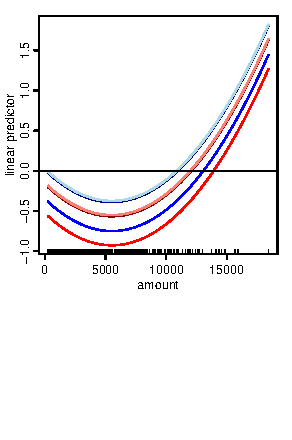
\includegraphics[width=5cm]{cd-amount-link-001} 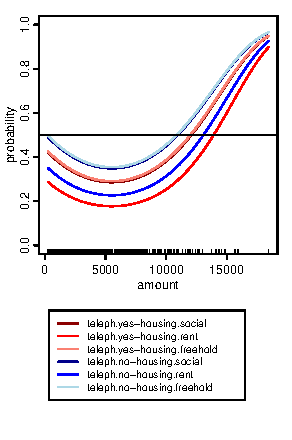
\includegraphics[width=5cm]{cd-amount-resp-001} 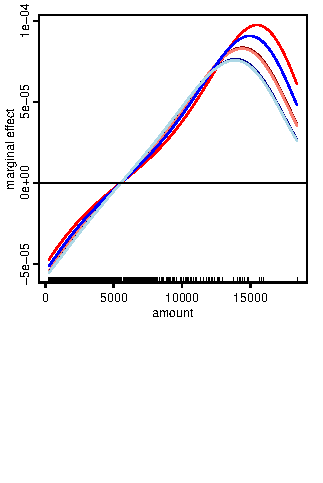
\includegraphics[width=5cm]{cd-amount-marg-001}
\vspace{-0.75cm}
\caption{Quadratic effects of the metric covariate \quotes{amount} in the linear predictor (left), the response (middle) and the marginal effect (right) in the 6 groups formed by the two factors \quotes{teleph} and \quotes{housing}. The other metric covariates are set to their means.} \label{fig-cd-amount}
\end{figure}

To allow more flexibility in the fit the metric covariate \quotes{amount} can  be included nonparametrically using a spline function. The modified function call is
%
\begin{Schunk}
\begin{Sinput}
 require("splines")
 model.2.fac.npamount <- glm(credit ~ bs(amount) + age + duration*teleph  
     + housing, family = binomial(link="probit"), data = creditdata)
 glm.interactive(model.2.fac.npamount) 
\end{Sinput}
\end{Schunk}
%
 
The resulting plots are shown in figure~\ref{fig-cd-amount-np}. For this plot the other metric covariates are set to their means.  Since the legend is identical to figure~\ref{fig-cd-amount} it is omitted here.

\begin{figure}[ht]
\centering
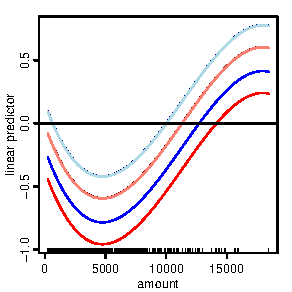
\includegraphics[width=5cm]{cd-amount-np-link-001} 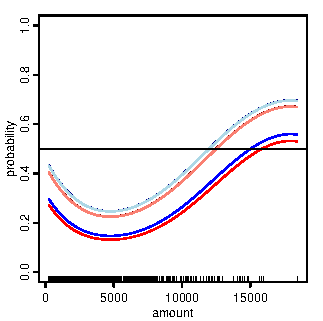
\includegraphics[width=5cm]{cd-amount-np-resp-001} 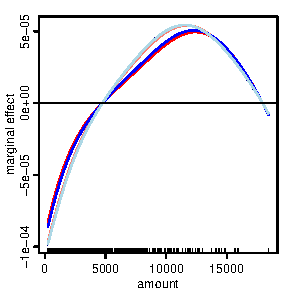
\includegraphics[width=5cm]{cd-amount-np-marg-001}
\caption{Nonparametric effect of the metric covariate \quotes{amount} in the linear predictor (left), the response (middle) and the marginal effect (right) in the 6 groups formed by the two factors \quotes{teleph} and \quotes{housing}. The other metric covariates are set to their means.} \label{fig-cd-amount-np}
\end{figure} 

\subsection{Interaction effects in binary response models}
The mechanics of interaction effects between metric and categorical covariates can easily be observed because in the termplots  every group is represented by an individual line. In the example model of section~\ref{sec-quickstart} there is an interaction between the metric covariate \quotes{duration} and the factor \quotes{teleph}. By choosing \quotes{duration} to be displayed this interaction effect can be observed directly in the linear predictors, the responses and the marginal effects. The corresponding plots are shown in figure \ref{fig-cd-dur-1}, for the plots the other metric covariates are left at their means.  The legend is identical to figure~\ref{fig-cd-amount} and therefore omitted.
\begin{figure}[ht]
\centering
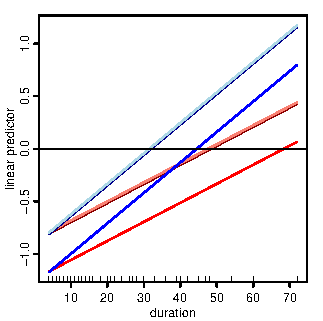
\includegraphics[width=5cm]{cd-dur-link-001} 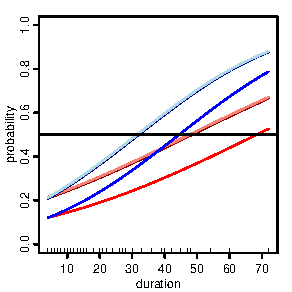
\includegraphics[width=5cm]{cd-dur-resp-001} 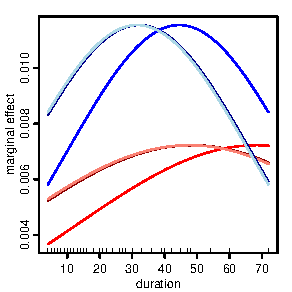
\includegraphics[width=5cm]{cd-dur-marg-001}
\caption{Direct visualization of the interaction effect between the metric covariate \quotes{duration} and the factor \quotes{teleph} in the linear predictor (left), the response (middle) and the marginal effect (right) in the 6 groups formed by the two factors \quotes{teleph} and \quotes{housing}. The other metric covariates are set to their means.} \label{fig-cd-dur-1}
\end{figure}

Due to the interactive nature of the functions the interaction effect becomes also visible when other covariates are selected to be displayed. The top row of  figure~\ref{fig-cd-age-1} shows the linear predictors, the responses and the marginal effects for the covariate \quotes{age}, the covariate  \quotes{amount} is left at the mean and the covariate \quotes{duration} is set to 12 months.  The legend is identical to figure~\ref{fig-cd-amount} and therefore omitted again. For the plots in the second row the covariate \quotes{duration} is set to 36 months. Due to the interaction effect the red lines are further away from the blue lines compared to the plots in the first row and by this the interaction effect becomes visible indirectly.

\begin{figure}[H]
\centering
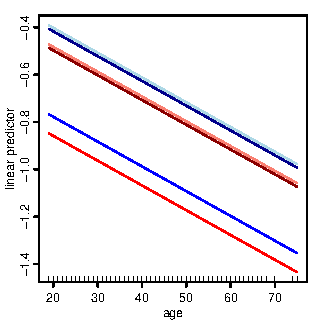
\includegraphics[width=5cm]{cd-age-link-1-001} 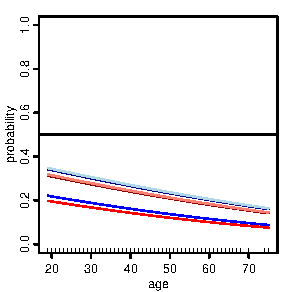
\includegraphics[width=5cm]{cd-age-resp-1-001} 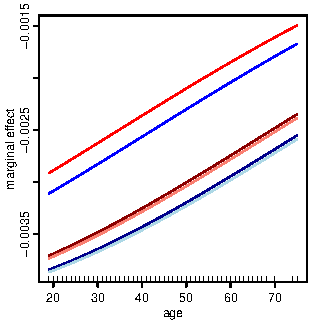
\includegraphics[width=5cm]{cd-age-marg-1-001}

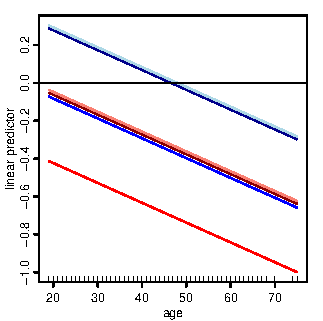
\includegraphics[width=5cm]{cd-age-link-2-001} 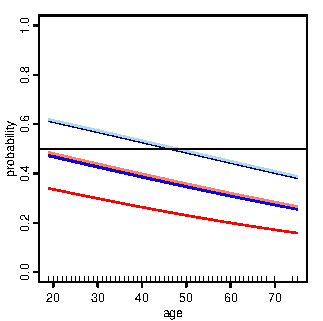
\includegraphics[width=5cm]{cd-age-resp-2-001} 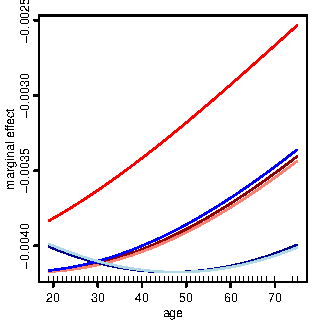
\includegraphics[width=5cm]{cd-age-marg-2-001}
\caption{Indirect visualization of the interaction effect between the metric covariate \quotes{duration} and the factor \quotes{teleph} in the linear predictor (left), the response (middle) and the marginal effect (right) of the metric covariate \quotes{age} in the 6 groups formed by the two factors \quotes{teleph} and \quotes{housing}. For the figures in the first row the covariate \quotes{duration} is set to 12 months and for the second row to 36 months, the covariate \quotes{amount} is set to the mean.} \label{fig-cd-age-1}
\end{figure}

\subsection{Uncover quasi-complete separation in binary response models}
This issue is discussed in Kleiber, Zeileis (2008), p. 130ff by means of the \code{MurderRates}-data which originate from a study on the deterrent effect of capital punishment in the USA in 1950. The authors uncover the problem of quasi-complete separation by tracing a suspiciously large standard deviation of the coefficient estimate for the dummy variable representing the level \quotes{yes} of the factor \quotes{southern}. It is pointed out that this issue is not uncommon with small data sets but is rarely discussed in textbooks and therefore can easily be overseen. Using \code{glm.interactive()}, choosing for instance the covariate \quotes{income} and selecting the probability termplot (see figure~\ref{fig-qcs}) directly reveals the source of the problem even for inexperienced users:
%
\begin{Schunk}
\begin{Sinput}
 require("AER")
 data("MurderRates")
 model <- glm(I(executions > 0) ~ time + income + noncauc + lfp + southern, 
     data = MurderRates, family = binomial)
 glm.interactive(model)
\end{Sinput}
\end{Schunk}
%

\begin{figure}[ht]
\centering
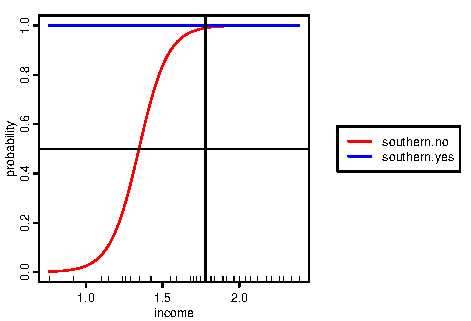
\includegraphics[width=7.5cm]{mr-income-resp-001}
\caption{The probability termplot of a metric covariate, here \quotes{income}, uncovers the quasi-complete separation in the \code{MurderRates}-data: Observations from the southern states are always predicted as 1.} \label{fig-qcs}
\end{figure}


\section{Details on the text output} \label{sec-output}
The example model from section~\ref{sec-quickstart} is used for illustration in this section with the metric covariates set to their means. The following tables are calculated and printed to the console by clicking the \emph{Snapshot}-button: 
\begin{itemize} [leftmargin=1cm, label=$\bullet$]
\item A summary of the model obtained by \code{summary()} (not shown).
\item Tables of the chosen values of the metric covariates and their ECDF-values (see table~\ref{tab-001}).

\begin{table}[ht]
\centering
\begin{minipage}[c]{8cm}
\begin{CodeChunk}
\small
\begin{CodeOutput}
Actual values of metric covariates
  amount      age duration 
3271.248   35.542   20.903 

ECDF of actual values of metric covariates
  amount      age duration 
   0.658    0.587    0.554
\end{CodeOutput}
\end{CodeChunk}
\end{minipage}
\caption{Tables of the chosen values of the metric covariates and their ECDF-values.} \label{tab-001}
\end{table}

\item For \code{glm.interactive()} the table of the link and response function evaluated for the chosen values of the metric covariates in each group (see table~\ref{tab-002}). For \code{lm.interactive()} the table of the effects for the chosen values of the metric covariates in each group.

\begin{table}[ht]
\centering
\begin{minipage}[c]{9cm}
\begin{CodeChunk}
\small
\begin{CodeOutput}
                                  link  response
teleph.yes-housing.social   -0.4988935 0.3089272
teleph.yes-housing.rent     -0.8599626 0.1949048
teleph.yes-housing.freehold -0.4843101 0.3140829
teleph.no-housing.social    -0.3219410 0.3737487
teleph.no-housing.rent      -0.6830100 0.2473003
teleph.no-housing.freehold  -0.3073576 0.3792856 
\end{CodeOutput}
\end{CodeChunk}
\end{minipage}
\caption{Table of the link and response function for the chosen values of the metric covariates in each group.} \label{tab-002}
\end{table}

\item Table of marginal effects for each metric covariate for the chosen values of the metric covariates 
in each group (see table~\ref{tab-003}). The marginal effects are calculated numerically with \code{splinefun()}.

\begin{table}[ht]
\centering
\begin{minipage}[c]{14cm}
\begin{CodeChunk}
\small
\begin{CodeOutput}
                            marg.eff.amount marg.eff.age marg.eff.duration
teleph.yes-housing.social     -2.092169e-05 -0.003687023       0.006380069
teleph.yes-housing.rent       -1.637025e-05 -0.002884925       0.004992109
teleph.yes-housing.freehold   -2.107222e-05 -0.003713551       0.006425974
teleph.no-housing.social      -2.249765e-05 -0.003964754       0.010967022
teleph.no-housing.rent        -1.876479e-05 -0.003306914       0.009147348
teleph.no-housing.freehold    -2.260112e-05 -0.003982988       0.011017462 
\end{CodeOutput}
\end{CodeChunk}
\end{minipage}
\caption{Table of marginal effects for each metric covariate for the chosen values of the metric covariates in each group.} \label{tab-003}
\end{table}
\end{itemize}

When the argument \code{latex2console} is set to \code{TRUE} in the function call the tables are printed to the console as \LaTeX-code. For the given example the tables \ref{tab-appendix-001} to \ref{tab-appendix-004} in the appendix show the results. Within a .tex-document the \LaTeX-code works with the following preamble, note that the \LaTeX-package \code{booktabs} is required:
\begin{Code}
\documentclass{scrartcl}
\usepackage{booktabs}
\begin{document}
% copy and paste from R Console
\end{document} 
\end{Code}

\section{Details on different aspects of usage} \label{sec-usage}
The arguments explained in this section control different aspects of usage. The model from section~\ref{sec-quickstart} is used as example and therefore the \code{glm.interactive()} is used throughout this section. For the \code{lm.interactive()} the arguments are identical.

\vspace{-0.3cm}\paragraph{Exact control over metric covariates} 
With the sliders the values of the metric covariates cannot be selected with arbitrary precision. To allow exact control over the values these can be set as initial values for the sliders with the argument \code{initial.values} through a named list. The names in the list must exactly match the variable names:
%
\begin{Schunk}
\begin{Sinput}
 glm.interactive(model.2.fac,
     initial.values = list(amount=5000, duration=24, age=30))
\end{Sinput}
\end{Schunk}
%

If a metric covariate is not explicitly listed the corresponding slider is initialized with the mean (the default). 

\vspace{-0.3cm}\paragraph{Preselect metric covariate, plot type and groups}
To avoid the appearance of a selection menu the name of the metric covariate to be displayed can be preselected:
%
\begin{Schunk}
\begin{Sinput}
 glm.interactive(model.2.fac, preselect.var = "duration")
\end{Sinput}
\end{Schunk}
%
If no metric covariate with the provided name exists the selection menu will pop up instead.

The type of plot to be displayed first can also be specified by the argument \code{preselect.type}. For the function \code{glm.interactive()} this must be one of the values \code{"link"} (the default), \code{"response"} or \code{"marginal"}: 
%
\begin{Schunk}
\begin{Sinput}
 glm.interactive(model.2.fac, preselect.type = "response")
\end{Sinput}
\end{Schunk}
%
For the function \code{lm.interactive()} the values \code{"effect"} (the default) and \code{"marginal"} are valid choices.

By default all groups are active in the initial plot. With the argument \code{preselect.groups} the groups  displayed in the initial plot can be specified by means of a 
numeric index vector. The first three groups are preselected by
%
\begin{Schunk}
\begin{Sinput}
 glm.interactive(model.2.fac, preselect.groups = c(1:3))
\end{Sinput}
\end{Schunk}
%
Preselecting groups is useful if the model contains many factors. In this case the panel usually grows beyond the screen and some groups are not accessible via the GUI-panel any more. The groups are constructed with the function \code{factor.combinations()} which can be used to identify groups of interest. This is illustrated in example B1 in appendix~\ref{sec-app-addexample}. 

The functionality to prespecify the variable, the plot type and certain groups in advance is beneficial when used in conjunction with the argument \code{initial.values} and the automatic save functionality. All taken together, this allows the reproduction of plots without user interaction, see the last example in this section.

\vspace{-0.3cm}\paragraph{Saving plots}
When the plot is saved as PDF- or EPS-file there is sometimes a problem concerning the width of the legend annotations. Depending on the font family and the fontsize in some cases the legend annotations do not fit into the box around the legend in the graphics file even though these do so in the graphics window. A workaround for this is to increase the width of the legend with the argument \code{legend.width.factor}, which is \code{1} by default. If this problem occurs the width of the legend can be increased about 10\% for instance by
%
\begin{Schunk}
\begin{Sinput}
 glm.interactive(model.2.fac, legend.width.factor = 1.1)
\end{Sinput}
\end{Schunk}
%


When the argument \code{snapshot.plot} is set to \code{TRUE} the current plot is saved to the working directory by \code{SavePlot()} when the \emph{Snapshot}-button is pressed. Note that in this case the \proglang{RGui}-window becomes the active window. The advantage to save plots this way instead of using the functionality of the \proglang{RGui} is the handling of the file name.  The file name can be specified in advance  by the argument \code{graphics.filename} and a hyphen followed by a sequential number with 3 digits is added to avoid that existing plots are overwritten. The path can also be specified within the filename. In addition the file format can be set by the argument \code{graphics.extension} which is passed to the \code{type}-argument in \code{SavePlot()} (default to \code{"pdf"}). To save plots of the covariate \quotes{duration} to the directory D:$\backslash$Temp by the \emph{Snapshot}-button one may use
%
\begin{Schunk}
\begin{Sinput}
 glm.interactive(model.2.fac, 
     preselect.var     = "duration",
     snapshot.plot     = TRUE,
     graphics.filename = "D:/Temp/fig-credprobit-duration")
\end{Sinput}
\end{Schunk}
%

By setting the argument \code{autosave.plot} to \code{TRUE} the initial plot is saved and the GUI-control is closed immediately after initialization. In conjunction with the 
arguments \code{initial.values}, \code{preselect.var}, \code{preselect.type} and \code{preselect.groups} this can be used to reproduce plots without user interaction. In case of the example model with 2 factors the plot of the marginal effects with a prespecified covariate constellation and a subset of the groups is saved to the actual working directory by
%
\begin{Schunk}
\begin{Sinput}
 glm.interactive(model.2.fac,
     initial.values      = list(amount=5000, duration=24, age=30), 
     preselect.var       = "duration",
     preselect.type      = "marginal",
     preselect.groups    = c(2,3,5,6),
     autosave.plot       = TRUE,
     graphics.filename   = "fig-credprobit-duration-marg",
     legend.width.factor = 1.05)
\end{Sinput}
\end{Schunk}
%

Note that the legend width needs to be increased here for the PDF-files to look as expected. The figures of section~\ref{sec-visualization} are created in this reproducible way, the code can be found in the \code{demo} of the package.  

\section{Details on customization} \label{sec-customization}
The appearance of the GUI-controls, the text output and the plots can be customized in many ways. The most important ones are demonstrated  for \code{glm.interactive()} in this section. For \code{lm.interactive()} most of the arguments are identical. If there are deviations this is explicitly mentioned. Two probit models are used for demonstration throughout this section. Firstly the model introduced in section~\ref{sec-quickstart}:
%
\begin{Schunk}
\begin{Sinput}
 data("creditdata")
 model.2.fac <- glm(credit ~ amount + I(amount^2)  + age + duration*teleph
     + housing, family = binomial(link="probit"), data = creditdata)
\end{Sinput}
\end{Schunk}
%
Additionally the following probit model with 3 metric covariates and 3 factors with 2, 3 and 4 levels respectively is also used occasionally:
%
\begin{Schunk}
\begin{Sinput}
 data("creditdata")
 model.3.fac <- glm(credit ~ amount + I(amount^2)  + age + duration*teleph 
     + housing + job, family = binomial(link="probit"), data = creditdata)
\end{Sinput}
\end{Schunk}
%

\subsection{Customize text output} \label{subsec-custom-text}

\vspace{-0.3cm}\paragraph{Separation characters in group names}
Within the group names which are used in the legend and the text output the character separating the factor name and the corresponding factor levels can be set with the argument \code{level.sep} (default to \quotes{.}). The character separating factor-factor level combinations can be set with the argument \code{factor.sep} (default to \quotes{-}). Another meaningful pair of separation characters is for instance
%
\begin{Schunk}
\begin{Sinput}
 glm.interactive(model.2.fac, 
     factor.sep = "|",
     level.sep  = ">")
\end{Sinput}
\end{Schunk}
%

\vspace{-0.3cm}\paragraph{Decimal mark and big mark in \LaTeX-output}
Changing the \LaTeX-output to continental European number formats can be achieved by 
%
\begin{Schunk}
\begin{Sinput}
 glm.interactive(model.2.fac,
     latex2console = TRUE,
     decimal.mark  = ",",
     big.mark      = ".")
\end{Sinput}
\end{Schunk}
%

For the \LaTeX-code printed to the console the following preamble (here prepared for German language) for a utf8-encoded TEX-file   works well:
\begin{Code}
\documentclass[a4paper]{scrartcl}
\usepackage[T1]{fontenc}
\usepackage[utf8]{inputenx}
\usepackage[ngerman]{babel}
\usepackage[babel,german=quotes]{csquotes}
\usepackage{icomma}
\usepackage{booktabs}
\begin{document}
% copy and paste from R Console}
\end{document}
\end{Code}

\vspace{-0.3cm}\paragraph{Scientific notation and number of digits}
The number of digits and the behaviour when to change to scientific notation in the text output (both plain text and \LaTeX-output) can be modified by the \proglang{R} options \code{digits} and \code{scipen}, see the documentation of \code{options()} for details. Changing the options in the \proglang{R Console} directly affects the format of the numbers and can therefore be modified between two clicks on the \emph{Snapshot}-button.


\subsection{Customize graphic device} \label{subsec-custom-graph}
Many graphical elements can be controlled directly by arguments in the function call. The major appearance of the plots can be controlled by manipulation of \code{par()}-arguments. If necessary graphical elements can be added to the plots by low-level plotting commands in the \proglang{R Console}. Note that elements added this way are not captured by the autosave functionality described at the end of section~\ref{sec-usage}. The example B2 in appendix~\ref{sec-app-addexample} shows how to save plots without user interaction in this case.

\vspace{-0.3cm}\paragraph{Plot dimensions and pointsize} The dimensions of the graphic device (in centimeters) and the pointsize of plotted text can be set. A more compact plot is obtained by:
%
\begin{Schunk}
\begin{Sinput}
 glm.interactive(model.2.fac, 
     dev.height       = 11,
     dev.width        = 11,
     dev.width.legend = 5,
     dev.pointsize    = 8) 
\end{Sinput}
\end{Schunk}
%

When a legend is added the overall width of the device is \code{dev.width} plus \code{dev.width.legend}. By default a legend is added when at least one factor is used as covariate. For more details on the legend refer to the paragraph \quotes{Legend} in this section.

\vspace{-0.3cm}\paragraph{Colours, line types and line widths}
The colours, line types and line widths for the line representing different groups in the plots and the legend can be set directly. For the model with 2 factors the following scheme is suitable:
%
\begin{Schunk}
\begin{Sinput}
 glm.interactive(model.2.fac, 
     lwd = rep(c(1,2),each=3),
     col = c(1,"blue",2))
\end{Sinput}
\end{Schunk}
%
Note that the arguments are recycled if necessary, in this case for the colour. The levels of the factor \quotes{teleph} are represented by the thickness of lines and the levels of the factor \quotes{housing} by the colour.
For the model with 3 factors one may use
%
\begin{Schunk}
\begin{Sinput}
 glm.interactive(model.3.fac,  
     lwd = rep(c(1,2), each=12),
     col = rep(c(1,"blue",2), each=4),  
     lty = c(1,2,3,4),
     dev.width.legend = 8)
\end{Sinput}
\end{Schunk}
%
The levels of the additional factor \quotes{job} are represented by the linetype here. The visual discrimination of 4 or more factors will be conceptually hard to achieve. In this case it may be advisable to display only a subset of groups by deselecting some of these in the checkbox or by using the argument \code{preselect.groups}. 

\vspace{-0.3cm}\paragraph{Title and axis labels}
By default no title is added to the plot, the label for the \emph{x}-axis is the name of the selected covariate and the label for the \emph{y}-axis is the name of the selected plot type. This can be overridden if necessary, for instance with more detailed annotations:
%
\begin{Schunk}
\begin{Sinput}
 glm.interactive(model.2.fac, 
     preselect.var  = "duration",
     preselect.type = "response",
     main           = "Interaction between 'duration' and factor 'teleph'",
     xlab           = "duration (months)",
     ylab           = "probability of credit default")
\end{Sinput}
\end{Schunk}
%

\vspace{-0.3cm}\paragraph{Legend}
A legend is added by default when at least one categorical covariate is used. The legend is plotted within an own region with the left and right margin of the legend region set to $0$. The legend frequently needs to be modified since the space required by the legend depends on the number of factors used as covariates, the lengths of the group names,  the physical screen resolution and the size of the \proglang{RGui}-window (if run in  MDI-mode, not relevant for users of \textbf{RStudio}). On the one hand the space for the legend itself can be modified and on the other hand the scaling of the legend. The first solution for the model with 3 factors is
%
\begin{Schunk}
\begin{Sinput}
 glm.interactive(model.3.fac, dev.width.legend = 8)
\end{Sinput}
\end{Schunk}
%
For the same model reducing the scale to 70\% of the original size also works:
%
\begin{Schunk}
\begin{Sinput}
 glm.interactive(model.3.fac, legend.cex = 0.7)
\end{Sinput}
\end{Schunk}
%
The position of the legend can be modified as well, refer to the documentation of \code{legend()} for details:
%
\begin{Schunk}
\begin{Sinput}
 glm.interactive(model.2.fac, legend.pos = "top")
\end{Sinput}
\end{Schunk}
%
With the argument \code{legend.width.factor} the width of the box around the legend can be manipulated, see the explanations in the paragraph \quotes{Save plots} in section \ref{sec-usage}.  

When factors are present the legend and the corresponding plot region for it can be completely suppressed by
%
\begin{Schunk}
\begin{Sinput}
 glm.interactive(model.2.fac, legend.add = FALSE)
\end{Sinput}
\end{Schunk}
%
Setting the additional argument \code{legend.space} to \code{TRUE} will create the  corresponding plot region without the legend:
%
\begin{Schunk}
\begin{Sinput}
 glm.interactive(model.2.fac,
     legend.add   = FALSE,
     legend.space = TRUE)
\end{Sinput}
\end{Schunk}
%

This can be useful if different plots are arranged in a document but for only one of the plots a legend should appear. The empty spaces ensure exact alignments and matching plot dimensions in this case. Figure~\ref{fig-cd-amount} in section~\ref{sec-visualization} is an example for this, the code to reproduce the figure can be found in the demo. To achieve full flexibility for the arrangement of plots in a document the legend can be plotted alone:
%
\begin{Schunk}
\begin{Sinput}
 glm.interactive(model.2.fac, legend.only = TRUE)
\end{Sinput}
\end{Schunk}
%
Note that in this case the width of the graphic device is solely controlled by  \code{dev.width.legend} and in conjunction with \code{dev.height} the overall size of the legend can be set precisely.

\vspace{-0.3cm}\paragraph{Rug plot}
By default a rug representation of the selected metric covariate is added to the southern axis of the plot. The length of the ticks can be controlled with the argument \code{rug.ticksize} which is \code{0.02} by default.  For many observations the rug considerably slows down the rebuild of the plot. Setting \code{rug.ticksize} to \code{0} or \code{NA} removes the rug representation:
%
\begin{Schunk}
\begin{Sinput}
 glm.interactive(model.2.fac, rug.ticksize = NA)
\end{Sinput}
\end{Schunk}
%
The colour of the rug tickmarks can be changed with the argument  \code{rug.col}:
%
\begin{Schunk}
\begin{Sinput}
 glm.interactive(model.2.fac, rug.col = "gray50")
\end{Sinput}
\end{Schunk}
%

If more detailed control over the rug is needed, the rug needs to be suppressed and added  with \code{rug()} from the \proglang{R Console}. The example B2 in section~\ref{sec-app-addexample} shows how to add a customized rug plot with transparent colours.

\vspace{-0.3cm}\paragraph{Vertical and horizontal lines}
To aid visual perception some straight lines are added to the plots by default. A vertical black line shows the actual value of the selected metric covariate. To suppress the vertical line, e.g. for printing the plot, use
%
\begin{Schunk}
\begin{Sinput}
 glm.interactive(model.2.fac, vline.actual = FALSE)
\end{Sinput}
\end{Schunk}
%

For \code{glm.interactive()} horizontal black lines are drawn in the plot of the linear predictor at height \code{0}, in the plot of the response at height \code{0.5} and in the plot of the marginal effect at height \code{0}  by default. These lines can be suppressed by setting the corresponding arguments to \code{NA}: 
%
\begin{Schunk}
\begin{Sinput}
 glm.interactive(model.2.fac,        
     pos.hline.link     = NA,   
     pos.hline.response = NA,   
     pos.hline.marginal = NA)   
\end{Sinput}
\end{Schunk}
%
With the same arguments the position of the lines can be changed. For the plot of the response this is reasonable if another probability threshold than $0.5$, say $0.56$, gives a better prediction accuracy:
%
\begin{Schunk}
\begin{Sinput}
 glm.interactive(model.2.fac, pos.hline.response = 0.56)
\end{Sinput}
\end{Schunk}
%

For the \code{lm.interactive()} the corresponding arguments are \code{pos.hline.effect} (default to \code{0}) and \code{pos.hline.marginal} (default to \code{0}). The appearance of the lines (solid black lines) cannot be changed by arguments. To modify the lines these must be suppressed and can be added with \code{abline()}-commands from the \proglang{R Console}. 

\vspace{-0.3cm}\paragraph{Number of points used for plotting} The effects are drawn for a sequence of equally spaced points over the span of the chosen metric covariate. With the argument \code{n.effects} the number of points can be controlled. If the lines of the effects are not smooth this value can be increased.  

\subsection{Predefining the graphic device} \label{subsec-predefine}
For more control over the appearance of the plots the graphic device can be specified in advance.
Two plot regions which can be accessed with high-level plotting commands are required. The legend is plotted first and the left and right margin of the legend region are set to $0$. In the following example the legend appears on the left side, the colours are specified via \code{palette()} and the margins as well as the scale of the text are changed. Note that for pointsize $10$ the width of the legend must be increased to achieve that the legend annotations fit into the box of the legend in the PDF-file.   
%
\begin{Schunk}
\begin{Sinput}
 windows(10,7, pointsize = 10)
 layoutmatrix <- matrix(c(1,2,2), 1, 3)
 layout(layoutmatrix)
 palette(c("darkred","red","salmon","darkblue","blue","lightblue"))
 par(cex = 1, mar = c(5,5,2,2)+0.1)
 glm.interactive(model.2.fac,
     preselect.var       = "amount",
     preselect.type      = "response",
     dev.defined         = TRUE,
     legend.width.factor = 1.1,
     snapshot.plot       = TRUE)
\end{Sinput}
\end{Schunk}
%

\subsection{Customize GUI-controls} \label{subsec-custom-gui}

\vspace{-0.3cm}\paragraph{Size of the GUI-controls} The size of the entire panel is calculated automatically and primarily depends on the number of covariates and groups. The layout of the panel can be modified by a number of parameters.  This can be useful for screens with a low resolution or if the model has a lot of groups. For the latter case the parameters are changed in the following example to save space:
%
\begin{Schunk}
\begin{Sinput}
 glm.interactive(model.3.fac,
     box.type.height           = 90, 
     box.group.character.width = 6, 
     box.group.line.height     = 25, 
     dist.obj.height           = 2)
\end{Sinput}
\end{Schunk}
%

Note that for a large number of groups not every group can be seen in the GUI-panel because the panel grows beyond the screen margin. In former versions of \pkg{rpanel} (< 1.1-3) the entries of the checkbox are squeezed together. Currently there is no way to circumvent this problem. At the moment the only solution is to choose the groups in advance using the argument \code{preselect.groups}, see the paragraph \quotes{Preselect metric covariate, plot type and groups} in section~\ref{sec-usage}.

\vspace{-0.3cm}\paragraph{Annotations of the GUI-controls} The annotations of the GUI-controls can be changed easily, for instance to German: 
%
\begin{Schunk}
\begin{Sinput}
 glm.interactive(model.2.fac,
     panel.title      = "Probit Modell",
     label.button     = "Schnappschuss",
     label.slider.act = "Dargestellte Variable: ",
     label.box.type   = "Typ",
     label.types      = c("Linearer Praediktor", "Wahrscheinlichkeit",
                          "Marginaler Effekt"),
     label.box.groups = "Gruppen")
\end{Sinput}
\end{Schunk}
%

For \code{lm.interactive()} the argument \code{label.types} is a character vector of length 2 for the two types of effect plots, the effects itself and the marginal effects.

\pagebreak

\section{Other fitted-model objects and problems with raw data extraction} \label{sec-call-classes}

\vspace{-0.3cm}\paragraph{Other classes of fitted-model objects}
For other classes of fitted-model objects than \class{glm} for the function \code{glm.interactive()} and \class{lm} for the \code{lm.interactive()} both functions may work as well. Technically there are two requirements for this:
\begin{enumerate}[leftmargin=1cm, rightmargin=0.5cm, label={\arabic{enumi}.}]
\item From the fitted-model object, say \code{model}, the raw data must be extractable with \code{get\_all\_} \code{vars(model\$terms, model\$data) } or \code{ get\_all\_vars(model\$terms,} \linebreak \code{model\$model)}. If there is a problem with the extraction of the raw data the workaround described in the next paragraph may help.
\item Appropriate prediction methods must exist. For \code{glm.interactive()} these are \code{predict(model, newdata, type = "link")} and \code{predict(model, newdata,} \linebreak \code{type = "response")}  and for \code{lm.interactive()} this is  \code{predict(model, newdata)}.  
\end{enumerate}
Of course the four prerequisites stated in section~\ref{sec-quickstart} must be met, too. 

For instance a fitted model object obtained by \code{gam()} from the package \pkg{gam} \citep{Hast2013} is compatible:
%
\begin{Schunk}
\begin{Sinput}
 data("creditdata")
 require("gam")
 model.gam <- gam(credit ~ s(amount) + lo(age) + duration*teleph + housing, 
         family = binomial, data = creditdata)
 glm.interactive(model.gam) 
\end{Sinput}
\end{Schunk}
%

A fitted-model object of the function \code{gam()} from the package \pkg{mgcv} \citep{Wood2014} works as well:
%
\begin{Schunk}
\begin{Sinput}
 data("creditdata")
 require("mgcv") 
 model.mgcv <- gam(credit ~ s(amount) + s(age) + duration*teleph + housing,  
     family = binomial, data = creditdata)
 glm.interactive(model.mgcv)
\end{Sinput}
\end{Schunk}
%
Note that for stability reasons the table of coefficients is usually omitted for other classes of fitted-model objects if the argument \code{latex2console} is set to \code{TRUE}.  

\vspace{-0.3cm}\paragraph{Solving problems with raw data extraction} Fitted-model objects of class \class{lm} lack a \code{data} slot. Therefore the raw data must be extractable with  
\code{get\_all\_vars(model\$terms, model\$model)}. For some formulas this extraction method does not work properly, for instance if a covariate is incorporated as spline function with \code{bs()}.  Adding  a \code{data} slot to the fitted-model object afterwards solves this particular problem. This is demonstrated by means of a linear regression model for the rents of apartments in Munich, Germany. The dataset \code{munichrent03} is contained in the package and was originally obtained from the \citet{DataRent2014}. The variables are described in the documentation of the dataset \code{munichrent03}:
%
\begin{Schunk}
\begin{Sinput}
 data("munichrent03")
 require("splines")
 model.rent <- lm(rent ~ bs(yearc) + area*location + upkitchen,
     data=munichrent03)
 model.rent$data <- munichrent03
 lm.interactive(model.rent)
\end{Sinput}
\end{Schunk}
%
Adding a \code{data} slot afterwards may also be helpful if the raw data cannot be extracted for other reasons.

%\bibliographystyle{jss}
%\bibliography{LinRegInteractive}

\begin{thebibliography}{10}
\newcommand{\enquote}[1]{``#1''}
\providecommand{\natexlab}[1]{#1}
\providecommand{\url}[1]{\texttt{#1}}
\providecommand{\urlprefix}{URL }
\expandafter\ifx\csname urlstyle\endcsname\relax
  \providecommand{\doi}[1]{doi:\discretionary{}{}{}#1}\else
  \providecommand{\doi}{doi:\discretionary{}{}{}\begingroup
  \urlstyle{rm}\Url}\fi
\providecommand{\eprint}[2][]{\url{#2}}

\bibitem[{Bowman \emph{et~al.}(2007)Bowman, Crawford, Alexander, and
  Bowman}]{BowmCrawAlex2007}
Bowman A, Crawford E, Alexander G, Bowman R (2007).
\newblock \enquote{\pkg{rpanel}: Simple Interactive Controls for \proglang{R}
  Functions Using the \pkg{tcltk} package.}
\newblock \emph{Journal of Statistical Software}, \textbf{17}(9), 1--18.

\bibitem[{Bowman \emph{et~al.}(2010)Bowman, Gibson, Scott, and
  Crawford}]{BowmGibsScot2010}
Bowman A, Gibson L, Scott M, Crawford E (2010).
\newblock \enquote{Interactive Teaching Tools for Spatial Sampling.}
\newblock \emph{Journal of Statistical Software}, \textbf{36}(13), 1--17.

\bibitem[{Dahl(2012)}]{Dahl2012}
Dahl DB (2012).
\newblock \emph{\pkg{xtable}: Export tables to LaTeX or HTML}.
\newblock \proglang{R} package version 1.7-0,
  \urlprefix\url{http://CRAN.R-project.org/package=xtable}.

\bibitem[{{Data Archive of the Department of Statistics, University of Munich
  and of the SFB 386}(2014{\natexlab{a}})}]{DataCred2014}
{Data Archive of the Department of Statistics, University of Munich and of the
  SFB 386} (2014{\natexlab{a}}).
\newblock \emph{Dataset ''Kreditscoring zur Klassifikation von
  Kreditnehmern''}.
\newblock
  \urlprefix\url{http://www.stat.uni-muenchen.de/service/datenarchiv/kredit/kredit.html}.

\bibitem[{{Data Archive of the Department of Statistics, University of Munich
  and of the SFB 386}(2014{\natexlab{b}})}]{DataRent2014}
{Data Archive of the Department of Statistics, University of Munich and of the
  SFB 386} (2014{\natexlab{b}}).
\newblock \emph{Dataset ''M\"unchner Mietspiegel 2003''}.
\newblock
  \urlprefix\url{http://www.stat.uni-muenchen.de/service/datenarchiv/miete/miete03.html}.

\bibitem[{Fox(2003)}]{Fox2003}
Fox J (2003).
\newblock \enquote{Effect Displays in \proglang{R} for Generalised Linear
  Models.}
\newblock \emph{Journal of Statistical Software}, \textbf{8}(15), 1--27.

\bibitem[{Hastie(2013)}]{Hast2013}
Hastie T (2013).
\newblock \emph{\pkg{gam}: Generalized Additive Models}.
\newblock \proglang{R}~package version~1.09.1,
  \urlprefix\url{http://CRAN.R-project.org/package=gam}.

\bibitem[{Hoetker(2007)}]{Hoet2007}
Hoetker G (2007).
\newblock \enquote{The Use of Logit and Probit Models in Strategic Management
  Research: Critical Issues.}
\newblock \emph{Strategic Management Journal}, \textbf{28}(4), 331--343.

\bibitem[{Wood(2014)}]{Wood2014}
Wood S (2014).
\newblock \emph{\pkg{mgcv}: Mixed GAM Computation Vehicle with GCV/AIC/REML
  Smoothness Estimation}.
\newblock \proglang{R}~package version~1.7-29,
  \urlprefix\url{http://CRAN.R-project.org/package=mgcv}.

\bibitem[{Xie(2013)}]{Xie2013}
Xie Y (2013).
\newblock \enquote{Animation: An R Package for Creating Animations and
  Demonstrating Statistical Methods.}
\newblock \emph{Journal of Statistical Software}, \textbf{53}(1), 1--27.

\end{thebibliography}


\pagebreak

\appendix
\section[Example of LaTeX text output]{Example of \LaTeX ~ text output}
The four tables together with the captions in this section are the default text output (see section~\ref{sec-output}) for the model given in section~\ref{sec-quickstart} with the argument \code{latex2console} set to \code{TRUE}. 

\vspace{-0.1mm}
\begin{table}[H]
\centering
\begin{tabular}{lrrrr} \toprule
 &  \multicolumn{1}{c}{Estimate} & \multicolumn{1}{c}{Std. Error} & \multicolumn{1}{c}{z value} & \multicolumn{1}{c}{Pr(>$|\mbox{z}|$)} \\ \midrule
(Intercept) & -2.856711e-01 & 2.452085e-01 & -1.16501299 & 0.2440137362 \\
amount & -1.456049e-04 & 5.318493e-05 & -2.73771078 & 0.0061868458 \\
I(amount\verb+^+2) & 1.317726e-08 & 3.910163e-09 & 3.37000201 & 0.0007516764 \\
age & -1.046677e-02 & 4.196524e-03 & -2.49415198 & 0.0126258471 \\
duration & 1.811182e-02 & 6.508570e-03 & 2.78276549 & 0.0053897748 \\
telephno & -4.964901e-02 & 1.900688e-01 & -0.26121597 & 0.7939259612 \\
housing.L & 1.031201e-02 & 1.220057e-01 & 0.08452066 & 0.9326424767 \\
housing.Q & 3.007653e-01 & 7.867191e-02 & 3.82303248 & 0.0001318204 \\
duration:telephno & 1.084062e-02 & 7.507286e-03 & 1.44401356 & 0.1487351600 \\
 \bottomrule 
\end{tabular}
\caption{Model coefficients} 
\label{tab-appendix-001}
\end{table}

\vspace{-1.7mm}
\begin{table}[H]
\centering
\begin{tabular}{lccc} \toprule
\multicolumn{1}{c}{variable}  &  \multicolumn{1}{c}{amount}  &  \multicolumn{1}{c}{age}  &  \multicolumn{1}{c}{duration} \\ \midrule 
\multicolumn{1}{c}{value}  & 3,271.248 & 35.542 & 20.903 \\ 
\multicolumn{1}{c}{ECDF(value)}  & 0.658 & 0.587 & 0.554 \\ \bottomrule 
\end{tabular}
\caption{Values of metric covariates where results are calculated} 
\label{tab-appendix-002}
\end{table}

\vspace{-1.7mm}
\begin{table}[H]
\centering
\begin{tabular}{lcc} \toprule
\multicolumn{1}{c}{groups} &  \multicolumn{1}{c}{link} & \multicolumn{1}{c}{response} \\ \midrule
teleph.yes-housing.social & -0.4988935 & 0.3089272 \\
teleph.yes-housing.rent & -0.8599626 & 0.1949048 \\
teleph.yes-housing.freehold & -0.4843101 & 0.3140829 \\
teleph.no-housing.social & -0.3219410 & 0.3737487 \\
teleph.no-housing.rent & -0.6830100 & 0.2473003 \\
teleph.no-housing.freehold & -0.3073576 & 0.3792856 \\
 \bottomrule 
\end{tabular}
\caption{Linear predictor and response in different groups for given values of metric covariates}
\label{tab-appendix-003}
\end{table}

\vspace{-1.7mm}
\begin{table}[H]
\centering
\begin{tabular}{lrrr} \toprule
 &  \multicolumn{1}{c}{amount} &  \multicolumn{1}{c}{age} &  \multicolumn{1}{c}{duration} \\ \midrule 
\multicolumn{1}{c}{value}  & 3,271.248 & 35.542 & 20.903 \\ 
\multicolumn{1}{c}{ECDF(value)}  & 0.658 & 0.587 & 0.554 \\ \midrule 
teleph.yes-housing.social & -2.092170e-05 & -3.687023e-03 & 6.380070e-03 \\ 
teleph.yes-housing.rent & -1.637027e-05 & -2.884925e-03 & 4.992110e-03 \\ 
teleph.yes-housing.freehold & -2.107224e-05 & -3.713551e-03 & 6.425975e-03 \\ 
teleph.no-housing.social & -2.249766e-05 & -3.964754e-03 & 1.096703e-02 \\ 
teleph.no-housing.rent & -1.876481e-05 & -3.306914e-03 & 9.147355e-03 \\ 
teleph.no-housing.freehold & -2.260113e-05 & -3.982988e-03 & 1.101747e-02 \\ 
 \bottomrule 
\end{tabular}
\caption{Marginal effects in different groups for given values of metric covariates}
\label{tab-appendix-004}
\end{table}

\section{Additional examples} \label{sec-app-addexample}

\vspace{-0.3cm}\paragraph{Example B1} For models with many groups the GUI-panel grows beyond the screen. The only way to select or deselect the nonvisible groups is to preselect these. In this example only the groups which occur more than 10 times in the data are choosen to be displayed.
%
\begin{Schunk}
\begin{Sinput}
 model.cd.manygroups <- glm(credit ~ amount + I(amount^2) + age 
     + duration*teleph + housing + intuse, family=binomial, data=creditdata)
 factor.combs       <- factor.combinations(creditdata[,c("teleph",
     "housing","intuse")])
 logic.index.groups <- factor.combs$counts > 10
 index.groups       <- seq(along=factor.combs$counts)[logic.index.groups]
 glm.interactive(model.cd.manygroups,
     preselect.var    = "amount",
     preselect.groups = index.groups)
\end{Sinput}
\end{Schunk}
%
\vspace{-0.3cm}\paragraph{Example B2} A customized rug plot with transparent colour is added by means of the low-level plotting command \code{segments()} and the result is saved to the current working directory.
%
\begin{Schunk}
\begin{Sinput}
 glm.interactive(model.2.fac, 
     preselect.var  = "amount",
     preselect.type = "response",
     rug.ticksize   = 0)
 segments(creditdata$amount, par("usr")[3], creditdata$amount, 
     par("fig")[3], col = rgb(0,0,0,0.2))
 savePlot("credidefault-customrug", "pdf") 
\end{Sinput}
\end{Schunk}
%

\section{Version history}

\begin{table}[ht]
\centering
\begin{tabular}{lll}
\toprule
Version & Date published & Changes                                           \\ \midrule
0.2-2   & 08.09.2014     & vignette revised \\
0.2-1   & 26.08.2014     & argument \texttt{preselect.groups} added          \\
        &                & argument \texttt{select.all.groups.begin removed} \\
        &                & problem with flickering plot solved         \\
        &                & no restrictions for the names of factors/factor levels any more \\
0.1-3   & 18.08.2014     & first published version                           \\ \bottomrule
\end{tabular} 
\end{table}
\end{document}
